\documentclass[10pt,fontset=fandol]{ctexart}

% CS336 assignment 讲义版式：letter + CM + 蓝/橙框
\newcommand{\reporoot}{../..}

\usepackage{lmodern}
\usepackage{amsmath,amssymb,bm}
\usepackage[letterpaper,margin=1in]{geometry}
\usepackage{xcolor}
\usepackage{booktabs}
\usepackage{caption}
\captionsetup{font=small, labelfont=bf, skip=4pt}
\usepackage{tikz}
\usetikzlibrary{arrows.meta,positioning,calc}
\usepackage{enumitem}
\usepackage{listings}
\usepackage{setspace}
\usepackage[most]{tcolorbox}
\usepackage{titlesec}
\usepackage{fancyhdr}
\usepackage{hyperref}

\definecolor{csblue}{RGB}{0,112,192}
\definecolor{csorange}{RGB}{230,126,34}
\definecolor{csteal}{RGB}{0,128,128}
\definecolor{csstring}{RGB}{46,139,87}
\colorlet{structurecolor}{csblue}
\colorlet{second}{csorange}

\hypersetup{
  colorlinks=true,
  linkcolor=red!70!black,
  urlcolor=csblue,
  citecolor=red!70!black,
  breaklinks=true,
  linktoc=all,
}
\setcounter{tocdepth}{2}

\IfFontExistsTF{DejaVu Sans Mono}{
  \setmonofont{DejaVu Sans Mono}[Scale=0.88]
}{}

\setlength{\parindent}{0pt}
\setlength{\parskip}{0.55em}
\setstretch{1.12}
\setlist{nosep, leftmargin=1.35em, itemsep=0.2em, topsep=0.35em}
\setlist[enumerate,1]{label=\arabic*.}
\setlist[itemize,1]{label=\textbullet}

\titleformat{\section}{\large\bfseries}{\thesection}{0.55em}{}
\titleformat{\subsection}{\normalsize\bfseries}{\thesubsection}{0.45em}{}
\titleformat{\subsubsection}{\normalsize\bfseries}{\thesubsubsection}{0.4em}{}
\titlespacing*{\section}{0pt}{1.35em}{0.4em}
\titlespacing*{\subsection}{0pt}{1.05em}{0.3em}
\titlespacing*{\subsubsection}{0pt}{0.85em}{0.25em}

\pagestyle{plain}
\fancyhf{}
\renewcommand{\headrulewidth}{0pt}
\cfoot{\thepage}

% 蓝框 = CS336 Low-Resource Tip；橙框 = Problem
\newcommand{\csboxline}{%
  \par\vspace{3pt}%
  \noindent{\color{black}\rule{\linewidth}{0.45pt}}\par
  \vspace{6pt}%
}
\newtcolorbox{csframe}[1]{
  colback=white,
  colframe=#1,
  boxrule=0.7pt,
  sharp corners,
  left=8pt, right=8pt, top=6pt, bottom=7pt,
  before skip=10pt, after skip=10pt,
}
\newenvironment{tipbox}[1]{%
  \begin{csframe}{csblue}%
  \noindent\textbf{#1}\csboxline
}{\end{csframe}}
\newenvironment{problembox}[1]{%
  \begin{csframe}{csorange}%
  \noindent\textbf{#1}\csboxline
}{\end{csframe}}

% 旧章命令映射到 article 节（正文仍写 \chapter / \section）
\let\textbooksection\section
\let\textbooksubsection\subsection
\NewDocumentCommand{\chapter}{s m}{%
  \IfBooleanTF{#1}{\textbooksection*{#2}}{\textbooksection{#2}}%
}
\RenewDocumentCommand{\section}{s m}{%
  \IfBooleanTF{#1}{\textbooksubsection*{#2}}{\textbooksubsection{#2}}%
}
\renewcommand{\subsection}{\subsubsection}
\renewcommand{\part}[1]{}
\providecommand{\frontmatter}{}
\providecommand{\mainmatter}{}
\renewcommand{\maketitle}{}

\newenvironment{introduction}{%
  \par\noindent\textbf{本讲要点}%
  \begin{itemize}%
}{\end{itemize}}
\newenvironment{note}{\begin{tipbox}{Note}}{\end{tipbox}}
\newenvironment{remark}{\begin{tipbox}{Remark}}{\end{tipbox}}
\newenvironment{conclusion}{\begin{tipbox}{Conclusion}}{\end{tipbox}}
\newenvironment{proposition}[1]{\begin{tipbox}{#1}}{\end{tipbox}}
\newenvironment{definition}[1]{\begin{tipbox}{#1}}{\end{tipbox}}
\newenvironment{runcmd}[1][怎么跑]{\begin{tipbox}{#1}}{\end{tipbox}}
\newenvironment{exercise}[1][]{\begin{problembox}{Problem#1}}{\end{problembox}}
\newenvironment{problemset}[1][]{%
  \begin{problembox}{#1}%
  \begin{enumerate}[label=(\alph*)]%
}{%
  \end{enumerate}%
  \end{problembox}%
}

\renewcommand{\arraystretch}{1.15}

\lstdefinestyle{pythoncode}{
  language=Python,
  basicstyle=\ttfamily\small,
  keywordstyle=\color{csteal},
  commentstyle=\color{black!45},
  stringstyle=\color{csstring},
  showstringspaces=false,
  breaklines=true,
  frame=none,
  numbers=none,
  tabsize=4,
  captionpos=b,
  columns=flexible,
  keepspaces=true,
  showlines=false,
  xleftmargin=0.6em,
}
\lstdefinestyle{shell}{
  language=Python,
  basicstyle=\ttfamily\small,
  keywordstyle=\color{csteal},
  commentstyle=\color{black!45},
  stringstyle=\color{csstring},
  breaklines=true,
  frame=none,
  numbers=none,
  columns=flexible,
  keepspaces=true,
  xleftmargin=0.6em,
}
\lstset{style=pythoncode}

\newcommand{\src}[4]{%
  \lstinputlisting[
    style=pythoncode,
    firstline=#2,
    lastline=#3,
    caption={#4},
  ]{\reporoot/#1}%
  \par\vspace{-0.3em}\noindent{\small 文件：\texttt{\detokenize{#1}:#2--#3}}%
}

\newcommand{\run}[1]{\texttt{\detokenize{#1}}}
\newcommand{\pyfile}[1]{\texttt{\detokenize{#1}}}
\providecommand{\kaishu}{}

\tikzset{
  opbox/.style={draw=csblue, thick, fill=csblue!8, inner sep=4pt, font=\small, align=center},
  sram/.style={draw=csorange, thick, fill=csorange!12, inner sep=4pt, font=\small, align=center},
  hbm/.style={draw=black!45, thick, fill=black!4, inner sep=4pt, font=\small, align=center},
  arr/.style={-Latex, csblue, thick},
  arrd/.style={-Latex, csorange, thick},
}
\newcommand{\fignote}[1]{\par\vspace{3pt}{\centering\small #1\par}\vspace{4pt}}
\graphicspath{{figures/}}
\newcommand{\facite}{Dao. \emph{FlashAttention-2: Faster Attention with Better Parallelism and Work Partitioning}. ICLR 2024}
\newcommand{\faurl}{https://arxiv.org/abs/2307.08691}
\newcommand{\paperfig}[3]{%
\begin{center}
\includegraphics[width=#2\linewidth]{#1}%
\fignote{#3}
\end{center}}
% 算子数据流图。先图后码。

\newcommand{\figmemhier}{%
\begin{center}
\begin{tikzpicture}[font=\small, node distance=0.7cm]
  \node[hbm, minimum width=7.2cm] (hbm) {HBM：大、慢。张量 $Q,K,V,O$ 住这里};
  \node[sram, minimum width=7.2cm, below=of hbm] (sram) {SRAM / 寄存器：小、快。tile 与 $(m,\ell)$ 住这里};
  \node[opbox, minimum width=7.2cm, below=of sram] (alu) {Tensor Core / ALU：\texttt{tl.dot}、\texttt{tl.sum}};
  \draw[arr] (hbm) -- (sram) node[midway, right=2pt] {load / store};
  \draw[arr] (sram) -- (alu);
\end{tikzpicture}
\fignote{换核改的是 HBM 往返和片上驻留，不是 Transformer 公式。}
\end{center}}

\newcommand{\figgpuhier}{%
\begin{center}
\begin{tikzpicture}[font=\small, node distance=0.5cm]
  \node[hbm, minimum width=8.6cm] (hbm) {HBM：整卡一份，张量住这里，往返最贵};
  \node[opbox, minimum width=8.6cm, below=of hbm] (l2) {L2：全芯片共享缓存};
  \node[sram, minimum width=8.6cm, below=of l2] (sm) {许多 SM：各有 SRAM（shared memory）、寄存器、Tensor Core};
  \node[opbox, minimum width=8.6cm, below=of sm] (wp) {一个 SM 上：硬件按 warp（32 线程、SIMT 锁步）调度};
  \draw[arr] (hbm) -- (l2);
  \draw[arr] (l2) -- (sm);
  \draw[arr] (sm) -- (wp);
\end{tikzpicture}
\fignote{一块 GPU $=$ 慢而大的 HBM $+$ 许多能独立干活的 SM。算子优化就是少碰 HBM、让 tile 留在 SM 上。}
\end{center}}

\newcommand{\figcudagrid}{%
\begin{center}
\begin{tikzpicture}[x=0.78cm,y=0.62cm,font=\small]
  \foreach \j in {0,1,2} {
    \draw[csblue, thick, fill=csblue!8] (\j*3.55, 0) rectangle ++(3.3, 2.35);
    \node at (\j*3.55+1.65, 2.0) {block \j};
    \foreach \t in {0,1,2,3} {
      \fill[csorange!40] (\j*3.55+0.22+\t*0.76, 0.28) rectangle ++(0.66, 0.85);
    }
    \node[font=\footnotesize] at (\j*3.55+1.65, 0.68) {threads};
  }
  \draw[csblue, thick] (-0.25,-0.45) rectangle (10.45,2.7);
  \node at (5.1, 3.15) {一次 \texttt{kernel<<<grid,block>>>} $=$ 一个 grid};
\end{tikzpicture}
\fignote{每个 block 落到一个 SM，块内线程共享 SRAM。CUDA 要你写「第 $t$ 号线程做什么」。}
\end{center}}

\newcommand{\figtritonabs}{%
\begin{center}
\begin{tikzpicture}[font=\small]
  \node[hbm, minimum width=4.3cm] (c) {CUDA：thread / warp};
  \node[opbox, minimum width=4.3cm, right=1.2cm of c] (t) {Triton：program $\approx$ block};
  \draw[arr] (c) -- (t);
\end{tikzpicture}
\fignote{编译器把 tile 摊到 warp。grid 和怎么分块仍要你定。}
\end{center}}

\newcommand{\figpidone}{%
\begin{center}
\begin{tikzpicture}[x=0.85cm,y=0.7cm,font=\small]
  \draw[csblue, thick] (0,0) rectangle (9,1.15);
  \draw[csblue] (3,0) -- (3,1.15);
  \draw[csblue] (6,0) -- (6,1.15);
  \fill[csblue!15] (0,0) rectangle (3,1.15);
  \node at (1.5,0.58) {block 0};
  \node at (4.5,0.58) {block 1};
  \node at (7.5,0.58) {block 2};
  \node[csblue] at (1.5,-0.4) {\texttt{pid}=0};
  \node[csblue] at (4.5,-0.4) {\texttt{pid}=1};
  \node[csblue] at (7.5,-0.4) {\texttt{pid}=2};
  \node at (4.5,1.6) {数组 $[0,\ldots,n-1]$};
\end{tikzpicture}
\fignote{一份 program 吃一块 \texttt{BLOCK}；尾巴用 \texttt{mask}。}
\end{center}}

\newcommand{\figtiletwo}{%
\begin{center}
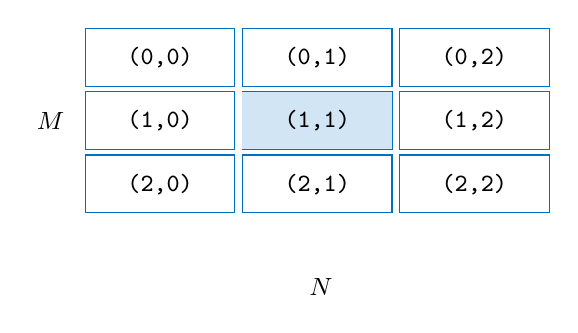
\begin{tikzpicture}[x=0.95cm,y=0.7cm,font=\small]
  \foreach \i in {0,1,2} {
    \foreach \j in {0,1,2} {
      \draw[csblue] (\j*2.1, -\i*1.15) rectangle ++(2.0,1.05);
      \node at (\j*2.1+1.0, -\i*1.15+0.52) {\texttt{(\i,\j)}};
    }
  }
  \fill[csblue!18] (2.1, -1.15) rectangle ++(2.0,1.05);
  \node at (3.1, -0.63) {\texttt{(1,1)}};
  \node[left] at (-0.15, -1.15+0.52) {$M$};
  \node at (3.15, -3.65) {$N$};
\end{tikzpicture}
\fignote{二维：\texttt{pid\_m} 管行块，\texttt{pid\_n} 管列块，各自乘 stride。}
\end{center}}

\newcommand{\figbandwidth}{%
\begin{center}
\begin{tikzpicture}[font=\small, node distance=1.15cm]
  \node[hbm] (x) {$x$};
  \node[hbm, right=of x] (y) {$y$};
  \node[sram, below=1.2cm of {$(x)!0.5!(y)$}] (alu) {$x+y$ 在片上};
  \node[hbm, below=of alu] (o) {out};
  \draw[arr] (x) -- (alu);
  \draw[arr] (y) -- (alu);
  \draw[arr] (alu) -- (o);
\end{tikzpicture}
\fignote{带宽绑定：一次加法，时间看两次 load、一次 store。}
\end{center}}

\newcommand{\figswiglu}{%
\begin{center}
\begin{tikzpicture}[font=\footnotesize, node distance=0.55cm]
  \node[align=center] at (2.2, 3.15) {\textbf{浅：中间 $a,b$ 进 HBM}};
  \node[hbm] (x1) at (0,2.2) {$x$};
  \node[hbm] (a1) at (2.0,2.55) {$a{=}xW_1$};
  \node[hbm] (b1) at (2.0,1.85) {$b{=}xW_2$};
  \node[hbm] (o1) at (4.4,2.2) {$\mathrm{SiLU}(a)\odot b$};
  \draw[arr] (x1) -- (a1);
  \draw[arr] (x1) -- (b1);
  \draw[arr] (a1) -- (o1);
  \draw[arr] (b1) -- (o1);
  \draw[dotted] (5.5,-0.15) -- (5.5,3.25);
  \node[align=center] at (8.6, 3.15) {\textbf{深：沿 $K$ 两次 dot}};
  \node[hbm] (x2) at (6.5,2.2) {$x$};
  \node[sram] (t2) at (8.6,2.2) {tile 上 $a,b$};
  \node[hbm] (o2) at (10.7,2.2) {out};
  \draw[arr] (x2) -- (t2);
  \draw[arr] (t2) -- (o2);
\end{tikzpicture}
\fignote{深融合少两次中间 GEMM 的 HBM 往返；大矩阵仍可能慢于 cuBLAS。}
\end{center}}

\newcommand{\figmatmul}{%
\begin{center}
\begin{tikzpicture}[x=0.48cm,y=0.48cm,font=\small]
  \draw[black!45, thick, fill=black!4] (0,1.6) rectangle (5.2,8.2);
  \fill[csblue!28] (0,4.4) rectangle (5.2,6.2);
  \node at (2.6,8.75) {$A$ $(M{\times}K)$};
  \node at (2.6,5.3) {$A_{ik}$};
  \draw[black!45, thick, fill=black!4] (7.2,5.6) rectangle (15.2,8.2);
  \fill[csblue!28] (9.6,5.6) rectangle (11.6,8.2);
  \node at (11.2,8.75) {$B$ $(K{\times}N)$};
  \node at (10.6,6.9) {$B_{kj}$};
  \draw[csorange, thick, fill=csorange!22] (9.6,1.8) rectangle (11.6,3.8);
  \node at (10.6,2.8) {$C_{ij}$};
  \draw[arr] (5.2,5.3) -- (9.55,3.1);
  \draw[arrd] (10.6,5.55) -- (10.6,3.9);
  \node[font=\footnotesize] at (7.6,4.15) {$\sum_k$};
  \node[font=\footnotesize] at (10.6,1.25) {SRAM 累加，沿 $K$ 循环};
\end{tikzpicture}
\fignote{一个 program 只写一块 $C$；归约维 $K$ 必须在核内 \texttt{for}，不能拆成不同 pid。}
\end{center}}

\newcommand{\figsoftmax}{%
\begin{center}
\begin{tikzpicture}[x=0.55cm,y=0.55cm,font=\small]
  \node at (4, 5.1) {\textbf{对：一行一个 pid}};
  \foreach \r in {0,1,2} {
    \draw[csblue] (0, 4-\r) rectangle (8, 4.85-\r);
    \fill[csblue!20] (0, 4-\r) rectangle (8, 4.85-\r);
    \node at (-1.15, 4.4-\r) {\texttt{pid}=\r};
    \node at (4, 4.4-\r) {$\max$ / $\mathrm{sum}$ 整行};
  }
  \begin{scope}[shift={(10.2,0)}]
    \node at (3.2, 5.1) {\textbf{错：把归约维切开}};
    \foreach \c in {0,1,2} {
      \draw[csorange] (\c*2.1, 2.2) rectangle ++(2.0, 2.5);
      \node at (\c*2.1+1.0, 3.45) {\texttt{pid}=\c};
    }
    \node[csorange, font=\footnotesize, align=center] at (3.15, 1.55) {各块的 max\\无法再合并};
  \end{scope}
\end{tikzpicture}
\fignote{归约维留下给核内 \texttt{for}；pid 只切独立的行（或 batch）。}
\end{center}}

\newcommand{\figonline}{%
\begin{center}
\begin{tikzpicture}[font=\small, node distance=0.85cm]
  \node[hbm] (x) {$x$ 一行};
  \node[sram, right=1.3cm of x] (s) {$(m,d)$};
  \node[hbm, right=1.3cm of s] (y) {$y$};
  \draw[arr] (x) -- node[above, font=\footnotesize] {第 1 趟} (s);
  \draw[arr] (s) -- node[above, font=\footnotesize] {第 2 趟} (y);
  \node[below=0.35cm of s, font=\footnotesize, align=center]
    {$m'=\max(m,m_{\mathrm{blk}})$\\$d'=d\,e^{m-m'}+d_{\mathrm{blk}}e^{m_{\mathrm{blk}}-m'}$};
\end{tikzpicture}
\fignote{online 统计量可合并，所以 Flash 能把 $K/V$ 留在内层循环。}
\end{center}}

\newcommand{\fignorm}{%
\begin{center}
\begin{tikzpicture}[x=0.5cm,y=0.5cm,font=\small]
  \foreach \r in {0,1,2} {
    \draw[csblue] (0, 3.2-\r*1.15) rectangle (7, 4.15-\r*1.15);
    \fill[csblue!12] (0, 3.2-\r*1.15) rectangle (7, 4.15-\r*1.15);
    \node at (3.5, 3.65-\r*1.15) {行 \r：$(\mu,\sigma)$ 本地};
  }
  \draw[csorange, thick] (8.2, 0.9) rectangle (13.4, 2.0);
  \node at (10.8, 1.45) {$\mathrm{d}\gamma,\mathrm{d}\beta$};
  \draw[arrd] (7.1, 3.65) -- (8.2, 1.7);
  \draw[arrd] (7.1, 2.5) -- (8.2, 1.55);
  \draw[arrd] (7.1, 1.35) -- (8.2, 1.4);
  \node[font=\footnotesize, align=left] at (10.8, 0.25) {\texttt{atomic\_add}};
\end{tikzpicture}
\fignote{$\mathrm{d}x$ 按行写；$\mathrm{d}\gamma/\mathrm{d}\beta$ 形状是 $(N,)$，多行必须原子加。}
\end{center}}

\newcommand{\fignaiveattn}{%
\begin{center}
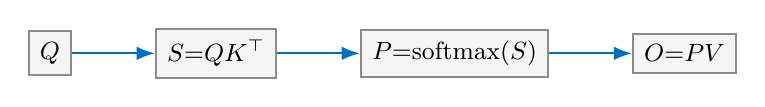
\begin{tikzpicture}[font=\small, node distance=1.05cm]
  \node[hbm] (q) {$Q$};
  \node[hbm, right=of q] (s) {$S{=}QK^\top$};
  \node[hbm, right=of s] (p) {$P{=}\mathrm{softmax}(S)$};
  \node[hbm, right=of p] (o) {$O{=}PV$};
  \draw[arr] (q) -- (s);
  \draw[arr] (s) -- (p);
  \draw[arr] (p) -- (o);
\end{tikzpicture}
\fignote{Naive：$S,P$ 是 $(S,S)$，写进 HBM。多头若 Host 串 launch，不是融合。}
\end{center}}

\newcommand{\figflashloop}{%
\begin{center}
\begin{tikzpicture}[x=1.05cm,y=0.78cm,font=\small]
  \foreach \j in {0,1,2,3} {\node at (\j+0.5, 3.55) {$K_{\j}$};}
  \foreach \i in {0,1,2} {
    \node at (-0.55, 2.45-\i) {$Q_{\i}$};
    \foreach \j in {0,1,2,3} {
      \fill[black!5] (\j, 2-\i) rectangle ++(0.95,0.85);
      \draw[black!40] (\j, 2-\i) rectangle ++(0.95,0.85);
    }
  }
  \fill[csorange!40] (0,1) rectangle ++(0.95,0.85);
  \fill[csorange!40] (1,1) rectangle ++(0.95,0.85);
  \draw[csorange, thick] (0,1) rectangle ++(0.95,0.85);
  \draw[csorange, thick] (1,1) rectangle ++(0.95,0.85);
  \node[sram, anchor=west, align=left] at (4.35, 1.42)
    {当前 $Q_1$\\SRAM $(m,\ell,\mathrm{acc})$\\没有 $S/P$};
  \node[font=\footnotesize] at (2.0, -0.35) {橙：内层正在扫的 $K$ 块};
\end{tikzpicture}
\fignote{Flash 双循环：外 $Q$ 可映射成 pid，内 $K/V$ 必须在同一 program 里扫。}
\end{center}}

\newcommand{\figcausal}{%
\begin{center}
\begin{tikzpicture}[x=0.48cm,y=0.48cm,font=\small]
  \foreach \i in {0,...,4} {
    \foreach \j in {0,...,4} {
      \ifnum\j>\i
        \fill[black!14] (\j, 5-\i) rectangle ++(1,1);
      \else
        \fill[csblue!40] (\j, 5-\i) rectangle ++(1,1);
      \fi
      \draw[black!35] (\j, 5-\i) rectangle ++(1,1);
    }
  }
  \draw[csorange, very thick] (1,3) rectangle (3,5);
  \node at (2.5, -0.45) {$K$ 列 $n$};
  \node[rotate=90] at (-0.65, 2.5) {$Q$ 行 $m$};
  \node[font=\footnotesize, align=left] at (8.9, 3.35)
    {蓝：$\texttt{offs\_n}\le\texttt{offs\_m}$\\灰：$-\infty$\\橙框：一块 $K$ 同时含过去和未来\\打在 \texttt{qk} 上，不是 load mask};
\end{tikzpicture}
\fignote{一块 $K$ 里常常同时有过去和未来，不能靠越界 mask 代替 causal。}
\end{center}}

\newcommand{\figfagrid}{%
\begin{center}
\begin{tikzpicture}[font=\small, node distance=0.35cm]
  \node[opbox, minimum width=5.4cm] (t) {教学：\texttt{grid=(B,H)}\\一个 program 扫完该头全部 $Q$};
  \node[sram, minimum width=5.4cm, below=0.7cm of t] (f) {加速：\texttt{grid=($S/B_M$, B, H)}\\一块 $Q$ 一个 program};
  \draw[arrd] (t) -- (f);
\end{tikzpicture}
\fignote{先读懂教学版的双循环，再看 Q 块并行和 GQA 的 \texttt{GROUP}。}
\end{center}}

\newcommand{\figlaunch}{%
\begin{center}
\begin{tikzpicture}[font=\small, node distance=0.45cm]
  \node[hbm, minimum width=5.6cm] (bad) {Host \texttt{for h}：每个头一次 launch};
  \node[opbox, minimum width=5.6cm, below=0.65cm of bad] (ok) {\texttt{grid=(B,H)}：一次 launch，$B{\times}H$ 个 program};
  \draw[arrd] (bad) -- (ok);
\end{tikzpicture}
\fignote{nsys 先数 kernel 名字和次数。Python 循环调核，时间线会被切碎。}
\end{center}}

\newcommand{\figtrainops}{%
\begin{center}
\begin{tikzpicture}[font=\small]
  \node[opbox, minimum width=6.4cm] (d) {默认 \texttt{fa}：只换注意力};
  \node[hbm, minimum width=6.4cm, below=0.7cm of d] (t) {对照 \texttt{fa,ln,swiglu}：教学 GEMM 常负优化};
  \draw[arr] (d) -- (t);
\end{tikzpicture}
\fignote{训练图里能换核，不等于该把所有层都换成教学实现。}
\end{center}}

\newcommand{\figgqa}{%
\begin{center}
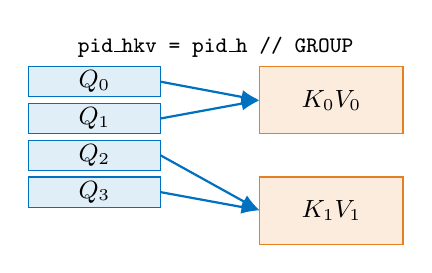
\begin{tikzpicture}[x=0.7cm,y=0.55cm,font=\small]
  \foreach \i in {0,1,2,3} {
    \draw[csblue, fill=csblue!12] (0, -\i*0.85) rectangle (2.4, 0.7-\i*0.85);
    \node at (1.2, 0.35-\i*0.85) {$Q_{\i}$};
  }
  \draw[csorange, fill=csorange!15] (4.2, -0.85) rectangle (6.8, 0.7);
  \node at (5.5, -0.08) {$K_0V_0$};
  \draw[csorange, fill=csorange!15] (4.2, -3.4) rectangle (6.8, -1.85);
  \node at (5.5, -2.62) {$K_1V_1$};
  \draw[arr] (2.4, 0.35) -- (4.2, -0.08);
  \draw[arr] (2.4, -0.5) -- (4.2, -0.08);
  \draw[arr] (2.4, -1.35) -- (4.2, -2.62);
  \draw[arr] (2.4, -2.2) -- (4.2, -2.62);
  \node[font=\footnotesize] at (3.4, 1.15) {\texttt{pid\_hkv = pid\_h // GROUP}};
\end{tikzpicture}
\fignote{GQA：$H_q>H_{kv}$。核里除法取 KV 头，不要 \texttt{repeat\_interleave}。}
\end{center}}



\begin{document}

\begin{center}
  {\LARGE\bfseries 用 Triton 写 GPU 算子}\\[0.45em]
  {\large 从 AI Infra 到训练对照}\\[0.85em]
  Version 0.1\\[0.15em]
  ai\_infra\\[0.15em]
  2026 年 9 月
\end{center}
\vspace{0.4em}

\tableofcontents
\vspace{0.8em}

\chapter*{前言}
\phantomsection
\addcontentsline{toc}{section}{前言}

\begin{introduction}
  \item 读者：会一点 Python / PyTorch
  \item 不需要 CUDA C++
  \item 用解释器跑 \texttt{.py}
  \item 环境：WSL2 + CUDA 12.8
  \item 算子章四块骨架
  \item 教学核常慢于库函数
\end{introduction}

这份讲义跟着仓库走：先写 kernel，再接到 generate 和若干步训练上。读者需要会一点 Python 和 PyTorch，不需要会 CUDA C++。

\section*{怎么用这本书}

正文分四部分。第一部分回答「为什么是 Triton」；第二部分按课号写算子；第三、四部分把核接到推理和训练。每一章算子尽量按同一骨架写：公式与数据流、怎么跑、正确性、效果。算子优化往往要靠数据流图才能看懂：\textbf{先看图里哪一维用 pid、哪一维必须核内 for、tile 住 HBM 还是 SRAM}，再对照摘录的代码。

\begin{note}
效果一节会反复强调：教学核常常慢于 \texttt{cuBLAS} / \texttt{SDPA}。课看的是分块、融合和 launch，不是端到端赢库函数。
\end{note}

完整程序在仓库里，书中只摘关键片段。路径相对于仓库根目录，例如

{\centering\pyfile{kernel/triton/tutorial/01_vector_add/step01_add_1d.py}\par}

\begin{runcmd}[启动方式]
跑示例请用解释器，不要把 \texttt{.py} 当 shell 脚本执行：
\begin{lstlisting}[style=shell]
cd /path/to/ai_infra
source .venv/bin/activate
python kernel/triton/tutorial/01_vector_add/step01_add_1d.py
\end{lstlisting}
\end{runcmd}

\section*{环境}

参考配置：RTX 5070 Laptop + WSL2。Blackwell（\texttt{sm\_120}）需要 \textbf{CUDA 12.8} 的 PyTorch 轮子。

\begin{runcmd}[本仓库环境]
\begin{lstlisting}[style=shell]
bash scripts/setup_env.sh
source .venv/bin/activate
\end{lstlisting}
\end{runcmd}

\begin{remark}
Windows 原生对 Triton 支持很弱，建议 Linux 或 WSL2。本机 \texttt{torch.profiler} 常常采不到 GPU，看 launch 用第~9~章的 \texttt{nsys}。作者进度板 \pyfile{kernel/triton/tutorial/学习计划书.md} 不是教材，附录只提炼其中仍然有效的坑。
\end{remark}

\chapter{从 AI Infra 到 Triton}

\begin{introduction}
  \item 训练 / 推理栈怎么分层
  \item 算子改的是 HBM 与 launch
  \item GPU：HBM / SM / warp
  \item CUDA：grid / block / thread
  \item Triton 在 CUDA 上抬了一层
  \item Triton 不替代 cuBLAS
\end{introduction}

写 kernel 之前，先看它落在训练/推理栈的哪一层，以及 GPU / CUDA 把并行切成哪几级。这一章几乎没有代码：把硬件、CUDA 的位置和 Triton 收掉了哪些细节说清楚，下一章再写 \texttt{pid} 与 \texttt{mask}。

\section{AI Infra 是什么}

大模型能跑起来，靠的不只是「Transformer 公式」。从用户请求到 GPU 上的一条指令，中间至少叠了这些层：

\begin{enumerate}
  \item \textbf{框架}：PyTorch 描述计算图、自动微分、混合精度。
  \item \textbf{编译器}：\texttt{torch.compile} / Inductor 把图收成更少的 kernel。
  \item \textbf{算子库}：cuBLAS、cuDNN、FlashAttention 等，把 GEMM、卷积、注意力做成高度特化的实现。
  \item \textbf{运行时与调度}：vLLM 这类系统做 PagedAttention、continuous batching、CUDA Graph，决定\textbf{何时}launch、launch \textbf{哪一批}请求。
  \item \textbf{硬件}：HBM、SRAM、Tensor Core、SM 数量。同一套公式，访存路径不同，墙钟差一个数量级并不罕见。
\end{enumerate}

\begin{proposition}{本仓库落在哪}
我们写的是第 3 层附近：\textbf{自己实现若干算子}，并接到一条 generate 和若干步训练上。不是造一个迷你 vLLM，也不追求端到端打败库函数。
\end{proposition}

\section{算子为什么重要}

同一套 Llama / Qwen 式结构里，时间往往耗在三类事情上：

\begin{itemize}
  \item 大矩阵乘（线性层、SwiGLU 的 gate/up/down）；
  \item 归一化（LayerNorm / RMSNorm）；
  \item 注意力（$QK^\top$、softmax、$PV$，以及 causal / GQA 变体）。
\end{itemize}

换核改变的是这一层的 \textbf{HBM 往返、片上 SRAM、launch 次数}，不是模型公式本身。

\figmemhier

教学核如果比 cuBLAS 慢，通常是 GEMM 形状已经够大、库函数吃满了 Tensor Core；这不说明「不该学分块」，只说明\textbf{对照对象要选对}。

\section{GPU 长什么样}

NVIDIA GPU 可以先看成两层：外面一份大而慢的内存，里面许多能并行干活的小核心。

\figgpuhier

\begin{itemize}
  \item \textbf{HBM}（全局内存）：容量大（十几到几十 GB），带宽相对片上仍慢。$Q,K,V,O$ 以及中间的 $S,P$ 默认住这里。
  \item \textbf{L2}：全芯片共享的缓存，课上不用手管。
  \item \textbf{SM}（Streaming Multiprocessor）：真正算的地方。每个 SM 有自己的 \textbf{shared memory}（SRAM，大约一百 KB 量级）、寄存器和 Tensor Core。一个 CUDA \textbf{block} 调度到其中一个 SM，块内线程才能共用这份 SRAM。
  \item \textbf{warp}：硬件调度单位，\textbf{32 条线程锁步}（SIMT）。Tensor Core 吃的是 warp 级的矩阵乘；一条线程跑到 \texttt{if}、另一条没跑到，就是 warp divergence。
\end{itemize}

\begin{proposition}{和算子的关系}
Flash 把 $S,P$ 留在 SRAM，是因为 HBM 往返比多算几次 softmax 统计量更贵。教学核 $D=512$ 跑不了，是因为这一份 tile 超过了单 SM 的 shared memory，不是公式错了。
\end{proposition}

\section{CUDA 的编程模型}

CUDA 把上面的硬件收成 Host 能启动的三级并行：

\figcudagrid

\begin{itemize}
  \item \textbf{grid}：一次 launch 的全部工作。Host 写 \texttt{kernel<<<grid, block>>>}。
  \item \textbf{block}：一份驻留在某个 SM 上的线程组，共享 SRAM，用 \texttt{\_\_syncthreads} 对齐。
  \item \textbf{thread}：你写的那一层。地址通常是 \texttt{blockIdx * blockDim + threadIdx}。
\end{itemize}

CUDA C++ 仍然是 NVIDIA GPU 上性能的底盘：warp、shared memory、occupancy、异步拷贝都可以直接管；cuBLAS / 官方 Flash 最终也是这一层。缺点是入门必须同时处理 thread 索引、同步、bank conflict 和 divergence。本课不写 CUDA C++，但后面的 \texttt{pid}、\texttt{BLOCK}、\texttt{num\_warps} 都是对着这张图说的。

\section{Triton 在 CUDA 上做了哪些抽象}

Triton 编译器的后端仍是 CUDA（PTX / cubin，同一套驱动）。它抬高的是\textbf{你要写到哪一层}。

\figtritonabs

\noindent\begin{minipage}{\linewidth}
\centering\small
\captionof{table}{Triton 收掉了什么、留下了什么}
\begin{tabular}{lll}
  \toprule
  & CUDA C++ & Triton \\
  \midrule
  并行单元 & thread / warp & program $\approx$ block \\
  区分实例 & \texttt{threadIdx} / \texttt{blockIdx} & \texttt{tl.program\_id} \\
  切一块数据 & 用线程号算偏移 & \texttt{BLOCK}+\texttt{arange}+\texttt{mask} \\
  块内同步 / SRAM & \texttt{\_\_shared\_\_}、\texttt{\_\_syncthreads} & 编译器插入 \\
  喂 Tensor Core & 自己排 warp / MMA & \texttt{tl.dot} \\
  几个 warp & \texttt{blockDim} & \texttt{num\_warps}（常 autotune） \\
  异步拷贝 & 自己写 & \texttt{num\_stages} \\
  启动 & \texttt{<<<grid,block>>>} & \texttt{kernel[grid](...)} \\
  \bottomrule
\end{tabular}
\end{minipage}

\begin{definition}{收掉 thread，不收掉分块}
Triton \textbf{不}替你决定哪一维用 pid、哪一维核内 \texttt{for}，也不替你决定中间结果住 HBM 还是 SRAM。融合、causal、GQA、launch 次数仍然是数据流问题。它收掉的是「第 $t$ 号线程怎么对齐、这块 tile 怎么摊到 4 个 warp 上」。
\end{definition}

所以：会 Triton 不是「不用懂 GPU」。HBM / SM / warp 这张骨架还在；只是你从 tile 往下看，不再从 thread 往上看。

\begin{definition}{Triton 不替代 CUDA}
教学核常常慢于 cuBLAS 和 SDPA。该调库函数的地方（大 GEMM、官方 Flash）课上仍调库。Triton 的价值是：\textbf{用可改的数据流把融合、causal、GQA、反向讲清楚}，并在需要时替换个别算子。
\end{definition}

对照如下。

\noindent\begin{minipage}{\linewidth}
\centering
\captionof{table}{三种写法各自管到哪一层}
\begin{tabular}{llll}
  \toprule
  & PyTorch eager & Triton & CUDA C++ \\
  \midrule
  并行单元 & 算子调用 & program / 块 & thread / warp \\
  典型作者 & 模型代码 & 算子数据流 & 硬件细节 \\
  和 autograd & 自动 & 需 \texttt{Function} & 需 \texttt{Function} + 更多样板 \\
  性能上限 & 依赖后端选择 & 中高（看形状） & 最高 \\
  本课用法 & 对照基线 & 主体 & 不写 \\
  \bottomrule
\end{tabular}
\end{minipage}

下一章从最小的向量加法开始，把 \texttt{pid}、\texttt{BLOCK}、\texttt{mask}、stride 写成可跑的套路。

\chapter{Triton 语法}

\begin{introduction}
  \item program / \texttt{pid} / \texttt{BLOCK} / \texttt{mask}
  \item 最小 \texttt{add\_kernel}
  \item stride 与二维广播
  \item \texttt{tl.dot}、归约、\texttt{atomic\_add}
  \item 常见坑
\end{introduction}

Triton 用类 Python 语法写 GPU kernel。第~1~章已经把 program 对上 CUDA block：你不写「第 $t$ 号线程处理一个元素」，而是：

\begin{proposition}{一块数据一份 program}
每个 \textbf{program}（$\approx$ 一个 CUDA block，落到一个 SM）一次处理一整块数据（\texttt{BLOCK\_SIZE} 个元素）。块内的 thread / warp 由编译器摊，\texttt{num\_warps} 只是提示。
\end{proposition}

\section{心智模型}

\begin{table}[htbp]
  \centering
  \caption{四个天天出现的词}
  \begin{tabular}{ll}
    \toprule
    概念 & 含义 \\
    \midrule
    program / \texttt{pid} & 并行执行的一份 kernel 实例，\texttt{tl.program\_id} 区分 \\
    \texttt{BLOCK\_SIZE} & 每个 program 一次处理多少元素，通常是 2 的幂 \\
    pointer + offset & 指针算术定位，再 \texttt{tl.load} / \texttt{tl.store} \\
    \texttt{mask} & 长度不是块整数倍时，多余位置不读不写 \\
    \bottomrule
  \end{tabular}
\end{table}

数据被切成多块，每个 \texttt{pid} 负责一块：

\figpidone

\section{最小完整程序}

套路只有四步：\texttt{pid}+\texttt{BLOCK} 得到 \texttt{offsets}；\texttt{mask}；load $\to$ 算 $\to$ store；Host 算 \texttt{grid} 并启动。仓库里可跑的版本如下（已挂 autotune，Host 不再传 \texttt{BLOCK\_SIZE}）。

\src{kernel/triton/tutorial/01_vector_add/step01_add_1d.py}{21}{48}{向量加法：kernel 与 Host 启动}

\begin{note}
\texttt{kernel[grid](...)} 按 grid 启动。\texttt{triton.cdiv(n, B)} 是向上取整。有 \texttt{@triton.autotune} 时不要再手传 \texttt{BLOCK\_*}，\texttt{grid} 用 \texttt{lambda meta}。
\end{note}

\section{Kernel 里能写什么}

\begin{itemize}
  \item \texttt{@triton.jit} 编译成 GPU kernel。里面只能用 \texttt{tl.*} 和受限 Python 子集，\textbf{不能}调 NumPy / PyTorch。
  \item 指针由 CUDA tensor 传入；长度等运行时标量每次可改；\texttt{BLOCK\_SIZE: tl.constexpr} 影响代码生成。
  \item 向量级选择用 \texttt{tl.where}，不要对每个元素写 Python \texttt{if}。编译期循环可用 \texttt{tl.static\_range}；Triton 里\textbf{没有} \texttt{break}。
\end{itemize}

二维 tile 的索引几乎总是广播：

\begin{lstlisting}[style=pythoncode, numbers=none]
offs_m = pid_m * BLOCK_M + tl.arange(0, BLOCK_M)
offs_n = pid_n * BLOCK_N + tl.arange(0, BLOCK_N)
offs  = offs_m[:, None] * stride_m + offs_n[None, :] * stride_n
mask  = (offs_m[:, None] < M) & (offs_n[None, :] < N)
\end{lstlisting}

\texttt{stride} 是「逻辑维 $+1$ 时内存跳几格」。地址 $=\mathrm{base}+\sum \mathrm{offs}_i\cdot\mathrm{stride}_i$。不要假设矩阵一定连续。

\figtiletwo

\section{常用原语}

累加器常用 FP32，即使输入是 BF16。矩阵乘的核心是 \texttt{tl.dot}。归约是 \texttt{tl.sum} / \texttt{tl.max}（Softmax、Norm、Attention 都会用）。多 program 往同一地址加，才用 \texttt{tl.atomic\_add}，并且 autotune 必须 \texttt{reset\_to\_zero}。

Host 侧计时用 \texttt{triton.testing.do\_bench}；对照前先 \texttt{torch.cuda.synchronize}，GEMM 对照请关掉 TF32。

\section{常见坑}

\begin{enumerate}
  \item 忘了 \texttt{mask}：越界读写。
  \item CPU tensor：必须 \texttt{device="cuda"}。
  \item 在 kernel 里用 PyTorch。
  \item FP16 累加不稳：归约用 FP32。
  \item 把 Python 动态 \texttt{list} 搬进 kernel。
\end{enumerate}

\begin{exercise}[建议顺序]
先向量加减 / ReLU，再行 Softmax，再小 matmul，再 fused bias+activation。官方教程：\url{https://triton-lang.org/main/getting-started/tutorials/index.html}。
\end{exercise}

\chapter{向量加法}

\begin{introduction}
  \item 一维 \texttt{mask}
  \item 二维 / 三维 stride
  \item 带宽绑定
  \item 文件：\texttt{01\_vector\_add/}
\end{introduction}

配套：\pyfile{kernel/triton/tutorial/01_vector_add/}。先跑：\pyfile{step01_add_1d.py} $\to$ \pyfile{step02_add_2d.py} $\to$ \pyfile{step03_add_3d.py}。

\section{公式与数据流}

\[
\mathrm{out}=x+y.
\]
每个 program 处理一块 \texttt{BLOCK} 元素；越界用 \texttt{mask}。二维、三维不要假设内存连续，用各自的 stride。二维 kernel 把 \texttt{pid} 拆成行块和列块：

\figtiletwo

\figbandwidth

\src{kernel/triton/tutorial/01_vector_add/step02_add_2d.py}{33}{47}{二维加法：stride 与二维 mask}

三维同理，再加一个 \texttt{pid} 轴。这是 launch 套路的操练场，不是算力测试。

\section{怎么跑}

\begin{runcmd}
\begin{lstlisting}[style=shell]
python kernel/triton/tutorial/01_vector_add/step01_add_1d.py
python kernel/triton/tutorial/01_vector_add/step02_add_2d.py
python kernel/triton/tutorial/01_vector_add/step03_add_3d.py
\end{lstlisting}
\end{runcmd}

\section{正确性}

\begin{note}
对照 \texttt{x + y}。elementwise 应对齐到 \texttt{atol} $10^{-5}$ 量级。
\end{note}

\section{效果}

\begin{remark}
这是\textbf{带宽绑定}：算的是一次加法，时间看 load/store。autotune 主要扫 \texttt{BLOCK} / \texttt{num\_warps}。不要拿它和 cuBLAS 比。
\end{remark}

\chapter{激活：ReLU 与 SwiGLU}

\begin{introduction}
  \item ReLU 前向 / 反向
  \item 浅 SwiGLU：HBM 上的 $a,b$
  \item 深融合：两次 \texttt{tl.dot}
  \item 反向重算 + cuBLAS GEMM
\end{introduction}

配套：\pyfile{kernel/triton/tutorial/02_activations/}。先跑：\pyfile{step01_relu.py} $\to$ \pyfile{step02_swiglu.py} $\to$ \pyfile{step03_swiglu_fused.py}。ReLU 只需第~2~章；深融合 SwiGLU 建议先扫一眼第~5~章 matmul（两次 \texttt{tl.dot}）。

\section{公式与数据流}

ReLU：
\[
y=\max(x,0),\qquad \mathrm{d}x=\mathrm{d}y\cdot\mathbf{1}_{x>0}.
\]
\texttt{tl.where(x > 0, x, 0.0)} 即可。反向在同文件 \texttt{TritonReLU}。

SwiGLU：
\[
\mathrm{out}=\mathrm{SiLU}(xW_1)\odot(xW_2),\qquad \mathrm{SiLU}(a)=a\cdot\sigma(a).
\]

\begin{itemize}
  \item \textbf{浅}（\pyfile{step02_swiglu.py}）：Host 上做两次 GEMM，kernel 只做 \texttt{silu(a)*b}，中间 $a,b$ 写 HBM。
  \item \textbf{深}（\pyfile{step03_swiglu_fused.py}）：同一 kernel 沿 $K$ 做两次 \texttt{tl.dot}，SiLU 与逐元乘之后写回，不物化 $a,b$。
\end{itemize}

\figswiglu

\src{kernel/triton/tutorial/02_activations/step03_swiglu_fused.py}{80}{114}{融合 SwiGLU：沿 K 两次 dot，再 SiLU 与乘}

\begin{proposition}{TritonSwiGLU 的反向}
正向是融合核；反向重算 $a,b$ 后，$\mathrm{d}W$ 仍走 PyTorch GEMM。这是教学接法，不是再写一个 TritonLinear。
\end{proposition}

\section{怎么跑}

\begin{runcmd}
\begin{lstlisting}[style=shell]
python kernel/triton/tutorial/02_activations/step01_relu.py
python kernel/triton/tutorial/02_activations/step02_swiglu.py
python kernel/triton/tutorial/02_activations/step03_swiglu_fused.py
\end{lstlisting}
\end{runcmd}

\section{正确性}

\begin{note}
ReLU / \texttt{TritonReLU} 对 \texttt{F.relu} 与 \texttt{autograd.grad}。SwiGLU 对 \texttt{silu(x@W1)*(x@W2)}；fp32 建议关 TF32，$\mathrm{rtol}=10^{-3}$。\texttt{TritonSwiGLU} 的 $\mathrm{d}x,\mathrm{d}W_1,\mathrm{d}W_2$ 对同一公式的 \texttt{autograd.grad}。
\end{note}

\section{效果}

\begin{remark}
深融合快在少两次中间 GEMM 的 HBM 往返。用 \texttt{do\_bench} 看 step02 vs step03。大矩阵上教学融合仍可能慢于 cuBLAS 两次 GEMM 再 elementwise——第~11~章训练默认因此不换 SwiGLU。
\end{remark}

\chapter{矩阵乘}

\begin{introduction}
  \item 输出块沿 $K$ 累加
  \item \texttt{reset\_to\_zero}
  \item 三维一次 launch
  \item \texttt{step90} 未收完，跳过
\end{introduction}

配套：\pyfile{kernel/triton/tutorial/03_matmul/}。先跑：\pyfile{step01_dot_1d.py} $\to$ \pyfile{step02_dot_3d.py} $\to$ \pyfile{step03_matmul_2d.py} $\to$ \pyfile{step04_matmul_3d.py}。

\begin{note}
选修 \pyfile{step90_linear_backward.py} \textbf{未收完}，初学者跳过。第~8~章 naive attention 会 import 三维 matmul。
\end{note}

\section{公式与数据流}

\[
C=A@B.
\]
每个 program 负责输出块 $(\texttt{BLOCK\_M},\texttt{BLOCK\_N})$，沿 $K$ 循环 \texttt{tl.dot} 累加。三维用 \texttt{pid\_b} 一次 launch，不要 Python \texttt{for b}。

\figmatmul

\src{kernel/triton/tutorial/03_matmul/step03_matmul_2d.py}{39}{64}{二维 matmul：输出块沿 K 累加}

一维点积把多块部分和 \texttt{atomic\_add} 到标量。autotune 若对同一输出累加，必须 \texttt{reset\_to\_zero}，否则 benchmark 污染结果：

\src{kernel/triton/tutorial/03_matmul/step01_dot_1d.py}{8}{35}{点积：atomic\_add 与 reset\_to\_zero}

对照是 \texttt{x @ w}。三维的 $w$ \textbf{不是} \texttt{F.linear} 的布局，不要混。

\section{怎么跑}

\begin{runcmd}
\begin{lstlisting}[style=shell]
python kernel/triton/tutorial/03_matmul/step01_dot_1d.py
python kernel/triton/tutorial/03_matmul/step03_matmul_2d.py
python kernel/triton/tutorial/03_matmul/step04_matmul_3d.py
\end{lstlisting}
\end{runcmd}

\section{正确性}

\begin{note}
关 \texttt{allow\_tf32} 再比。fp32 下看 max abs err，不要用带 bias 的 \texttt{F.linear} 当三维对照。
\end{note}

\section{效果}

\begin{remark}
教学核通常慢于 cuBLAS。课看的是分块数据流：哪一维 \texttt{pid} 并行、哪一维 kernel 内 \texttt{for}。后面 Flash 的 $QK^\top$ 就是反复调用这一套 \texttt{tl.dot}。
\end{remark}

\chapter{Softmax}

\begin{introduction}
  \item 归约维不能用 \texttt{pid} 切开
  \item Naive 整行
  \item Online：为 Flash 铺路
  \item 反向 $\mathrm{d}x=y(\mathrm{d}y-\sum y\,\mathrm{d}y)$
\end{introduction}

配套：\pyfile{kernel/triton/tutorial/04_softmax/}。先跑：\pyfile{step01_naive.py} $\to$ \pyfile{step02_online.py}。选修反向：\pyfile{step90_backward.py}。

\section{公式与数据流}

对最后一维：
\[
m=\max_j x_j,\qquad y_j=\frac{e^{x_j-m}}{\sum_k e^{x_k-m}}.
\]

\begin{proposition}{归约维}
归约维不能用 \texttt{program\_id} 切开：要么整行装下，要么 program 内 \texttt{for} 分块合并统计量。
\end{proposition}

\figsoftmax

Naive：一个 program 处理若干行，\texttt{BLOCK\_COLS} 覆盖整行。

\src{kernel/triton/tutorial/04_softmax/step01_naive.py}{46}{75}{Naive 行 Softmax：整行 max / sum}

Online：沿列分块维护可合并的 $(m,d)$，
\[
m'=\max(m,m_{\mathrm{blk}}),\quad
d'=d\,e^{m-m'}+d_{\mathrm{blk}}e^{m_{\mathrm{blk}}-m'}.
\]
两趟扫描：先得到全局 $(m,d)$，再写 $y=e^{x-m}/d$。这是为 $N$ 很大，以及后面 Flash 的在线 softmax 做准备。

\figonline

\src{kernel/triton/tutorial/04_softmax/step02_online.py}{50}{77}{Online Softmax：两趟列块}

反向（存 $y$ 不存 $x$）：
\[
\mathrm{d}x=y\odot\bigl(\mathrm{d}y-\langle y,\mathrm{d}y\rangle\mathbf{1}\bigr).
\]
\texttt{TritonSoftmax.apply} 才建图；裸 \texttt{naive\_softmax} 没有 \texttt{grad\_fn}。

\src{kernel/triton/tutorial/04_softmax/step90_backward.py}{109}{160}{反向闭式与 Function}

\section{怎么跑}

\begin{runcmd}
\begin{lstlisting}[style=shell]
python kernel/triton/tutorial/04_softmax/step01_naive.py
python kernel/triton/tutorial/04_softmax/step02_online.py
python kernel/triton/tutorial/04_softmax/step90_backward.py
\end{lstlisting}
\end{runcmd}

\section{正确性}

\begin{note}
对 \texttt{F.softmax(..., dim=-1)}；反向 \texttt{autograd.grad}。入门形状最后一维先 $\le 1024$。
\end{note}

\section{效果}

\begin{remark}
完整写出 $y$ 时，online \textbf{不一定更快}（多读一遍 $x$）。意义是 $N$ 装不进寄存器，以及给 Flash 准备 $(m,\ell)$ 这类统计量。
\end{remark}

\chapter{LayerNorm 与 RMSNorm}

\begin{introduction}
  \item LN vs RMS
  \item 行统计量
  \item $\mathrm{d}\gamma/\mathrm{d}\beta$ 用 \texttt{atomic\_add}
  \item 推理 API 是 \texttt{rmsnorm}
\end{introduction}

配套：\pyfile{kernel/triton/tutorial/05_norm/}。先跑：\pyfile{step01_layernorm.py} $\to$ \pyfile{step02_online_layernorm.py} $\to$ \pyfile{step03_rmsnorm.py}。推理 Host API 是 \texttt{from step03\_rmsnorm import rmsnorm}。LN 反向写在 step01 同文件。

\section{公式与数据流}

LayerNorm（最后一维 $N$）：
\[
\hat x=\frac{x-\mu}{\sqrt{\sigma^2+\varepsilon}},\qquad
y=\gamma\odot\hat x+\beta.
\]
RMSNorm 没有减均值、没有 $\beta$：
\[
\mathrm{rms}=\sqrt{\mathrm{mean}(x^2)+\varepsilon},\qquad
y=w\odot x/\mathrm{rms}.
\]

Naive LN 把整行 $N$ 一次装下。$N$ 很大时会炸寄存器；online 沿 $N$ 分块累加 $\sum x$、$\sum x^2$。

\fignorm

\src{kernel/triton/tutorial/05_norm/step01_layernorm.py}{69}{81}{LayerNorm 前向：行均值、方差、仿射}

反向里 $\mathrm{d}x$ 每行本地可写；$\mathrm{d}\gamma,\mathrm{d}\beta$ 形状是 $(N,)$，要把所有行加在一起。本块先 \texttt{sum(axis=0)}，再 \texttt{atomic\_add} 到全局。autotune 必须 \texttt{reset\_to\_zero}。

\src{kernel/triton/tutorial/05_norm/step01_layernorm.py}{223}{227}{参数梯度：tile 内求和再原子加}

\section{怎么跑}

\begin{runcmd}
\begin{lstlisting}[style=shell]
python kernel/triton/tutorial/05_norm/step01_layernorm.py
python kernel/triton/tutorial/05_norm/step02_online_layernorm.py
python kernel/triton/tutorial/05_norm/step03_rmsnorm.py
\end{lstlisting}
\end{runcmd}

\section{正确性}

\begin{note}
LN 对 \texttt{F.layer\_norm}。RMS 对 \texttt{F.rms\_norm}。fp32，$\mathrm{rtol}$ 约 $10^{-4}$。训练必须 \texttt{TritonLayerNorm.apply}，不能对裸 \texttt{layernorm(...)} 求 \texttt{grad}。
\end{note}

\section{效果}

\begin{remark}
大 $N$ 时分块版接近 torch，是因为 naive 整行会炸寄存器，不是因为公式更快。教学 LN 大 hidden 仍打不过 \texttt{F.layer\_norm}（背后是 cuDNN），训练默认不换它。
\end{remark}

\chapter{注意力：从 Naive 到 Flash}

\begin{introduction}
  \item Naive / MHA 是 Host 串
  \item 单头 Flash：论文双循环
  \item 教学多头 causal：\texttt{grid=(B,H)}
  \item 加速版：Q 块并行与 GQA
  \item RoPE / GQA / MLA
\end{introduction}

配套：\pyfile{kernel/triton/tutorial/06_attention/}。先跑：naive $\to$ MHA $\to$ 单头 Flash $\to$ \textbf{教学多头 causal} $\to$ RoPE $\to$ GQA。加速版 \pyfile{step04_flash_causal_mha.py} 给训练用；对照课请先读教学版。MLA 选修。Qwen3.5 的 DeltaNet 本课不实现。

\section{Naive 与多头：Host 串起来不算融合}

单头：
\[
S=\frac{QK^\top}{\sqrt{d}},\quad
P=\mathrm{softmax}(S),\quad
O=PV.
\]
$S,P$ 是 $(S,S)$，写进 HBM。多头把 $(B,H,S,d)$ 展成 $(BH,S,d)$ 再调三维 matmul。这是 Host 上多次 launch，\textbf{不是} kernel 融合。

\fignaiveattn

\begin{proposition}{对照}
对照用 \texttt{F.scaled\_dot\_product\_attention}（\texttt{is\_causal=True}）。不要用带投影的 \texttt{multi\_head\_attention\_forward}。SDPA 会选后端，不等于「一次 Flash」。
\end{proposition}

\section{单头 Flash：论文双循环}

数据流以 FlashAttention-2 论文为准（\facite；\url{\faurl}）。要点：外层 $Q$ 行块、内层 $K/V$ 列块，片上维护 $(m,\ell,\mathrm{acc})$，不把 $S/P$ 写回 HBM。外层可以映射成 \texttt{program\_id}，内层\textbf{必须} \texttt{for}——online 统计量不能按列拆成不同 program。

论文 Fig.~1 把「切 $K/V$、片上 softmax、用 $\ell$ 重标定 $O$」画在一张图里。蓝实线框在 HBM，橙虚线框在 SRAM（不物化）：

\paperfig{fa2-fig1-tiling.png}{0.98}{论文 Fig.~1：\facite。$K,V$ 切成两块时，先算 $(S^{(1)},A^{(1)},O^{(1)})$，再与第二块用 $\ell$ 重标定得到正确的 $O$。}

课上把同一件事收成「谁是 pid、谁必须核内 for」：

\figflashloop

论文 Algorithm~1 就是这层双循环。外 $i$ 扫 $Q$ 块（我们的 \texttt{BLOCK\_M}），内 $j$ 扫 $K/V$ 块（\texttt{BLOCK\_N}），片上更新 $m_i,\ell_i,O_i$，最后写 $O_i$ 和 $\mathrm{LSE}_i=m_i+\log\ell_i$：

\paperfig{fa2-alg1-forward.png}{0.96}{论文 Algorithm~1：FlashAttention-2 前向。教学单头把两层 \texttt{for} 都留在核里，方便一行行对照。}

教学单头 \texttt{grid=(B,)}，双重 \texttt{for} 都在核内：

\src{kernel/triton/tutorial/06_attention/step03_flash_single.py}{83}{114}{单头 Flash：外 Q 内 KV}

\begin{proposition}{shared memory}
Head dim $D$ 保持 64/128。把 hidden$=512$ 当一头会让 $(\texttt{BLOCK\_M},D)$ 爆 shared memory。本机 smem 上限大约 $101376$ 字节；教学核把整段 $D$ 放进 SRAM，$D=512$ 会跑不了。
\end{proposition}

\section{教学多头 causal}

文件：\pyfile{step04_flash_causal_mha_teach.py}。\\
\texttt{grid=(B,H)}，一个 program 一个头，内部仍是论文双循环。Causal 打在 \texttt{qk} 上：\texttt{offs\_n <= offs\_m} 才保留，否则 $-\infty$。这不是 \texttt{tl.load} 的越界 mask；$K/V$ 块里常常同时含过去和未来。

\figcausal

正向必须写下
\[
\mathrm{LSE}_i=m_i+\log \ell_i,
\]
形状 $(B,H,S)$，反向用 $\mathrm{P}_{ij}=\exp(S_{ij}-\mathrm{LSE}_i)$ 重算，不能存完整 $P$。

反向教学布局：\textbf{外层 KV 列块}（本地攒 $\mathrm{d}K/\mathrm{d}V$），\textbf{内层 Q 行块}（$\mathrm{d}Q$ 用 \texttt{atomic\_add}）。因此 Host 上 \texttt{dQ} 必须 \texttt{zeros\_like}，不能 \texttt{empty}。这就是论文 Fig.~2 右边：每个 worker 负责注意力矩阵的一列块。

\src{kernel/triton/tutorial/06_attention/step04_flash_causal_mha_teach.py}{70}{91}{教学 FA：grid 是 (B,H)，外层 for 扫 Q 块}

\begin{note}
数值对照必须走 \texttt{TritonFlashAttentionCausalMHA.apply}，不能对裸 Triton 的 $O$ 求 \texttt{grad}。一次 \texttt{grad(o,(q,k,v),do)} 求出三个梯度。
\end{note}

\section{加速版：训练在用的核}

文件：\pyfile{step04_flash_causal_mha.py}。相对教学版，核心是把论文 Fig.~2 的并行做进去：前向每个 worker 一行块（一块 $Q$），反向每个 worker 一列块（一块 $K/V$，$dQ$ 原子加）。

\paperfig{fa2-fig2-parallel.png}{0.82}{论文 Fig.~2：\facite。左：前向按行块并行（加速版的 Q 块 pid）。右：反向按列块并行（教学反向的 KV 外层）。}

\figfagrid

\begin{enumerate}
  \item \textbf{Q 块并行}：\texttt{grid=(cdiv(S, BLOCK\_M), B, H)}，每个 program 一块 $Q$。
  \item \textbf{GQA}：\texttt{GROUP=H\_q/H\_{kv}}，\texttt{pid\_hkv = pid\_h // GROUP}，不再 \texttt{repeat\_interleave} KV。
  \item Causal 用循环上界收掉未来 KV 块（Triton 不能 \texttt{break}）。
  \item 反向改成 Q 并行：本地写 $\mathrm{d}Q$，对 $\mathrm{d}K/\mathrm{d}V$ \texttt{atomic\_add}（fp32 累加）。
\end{enumerate}

论文 Fig.~3 是\textbf{同一个 thread block 里} warp 怎么切。FlashAttention 切 $K/V$（split-K，中间结果要进 shared memory 再加）；FlashAttention-2 改切 $Q$，各 warp 自己写出对应的 $O$ 片，少一次 smem 同步。Triton 的 \texttt{tl.dot} 不让你直接排 warp，但这解释了官方 FA2 为什么比 FA1 快。

\begin{center}
\begin{tabular}{@{}cc@{}}
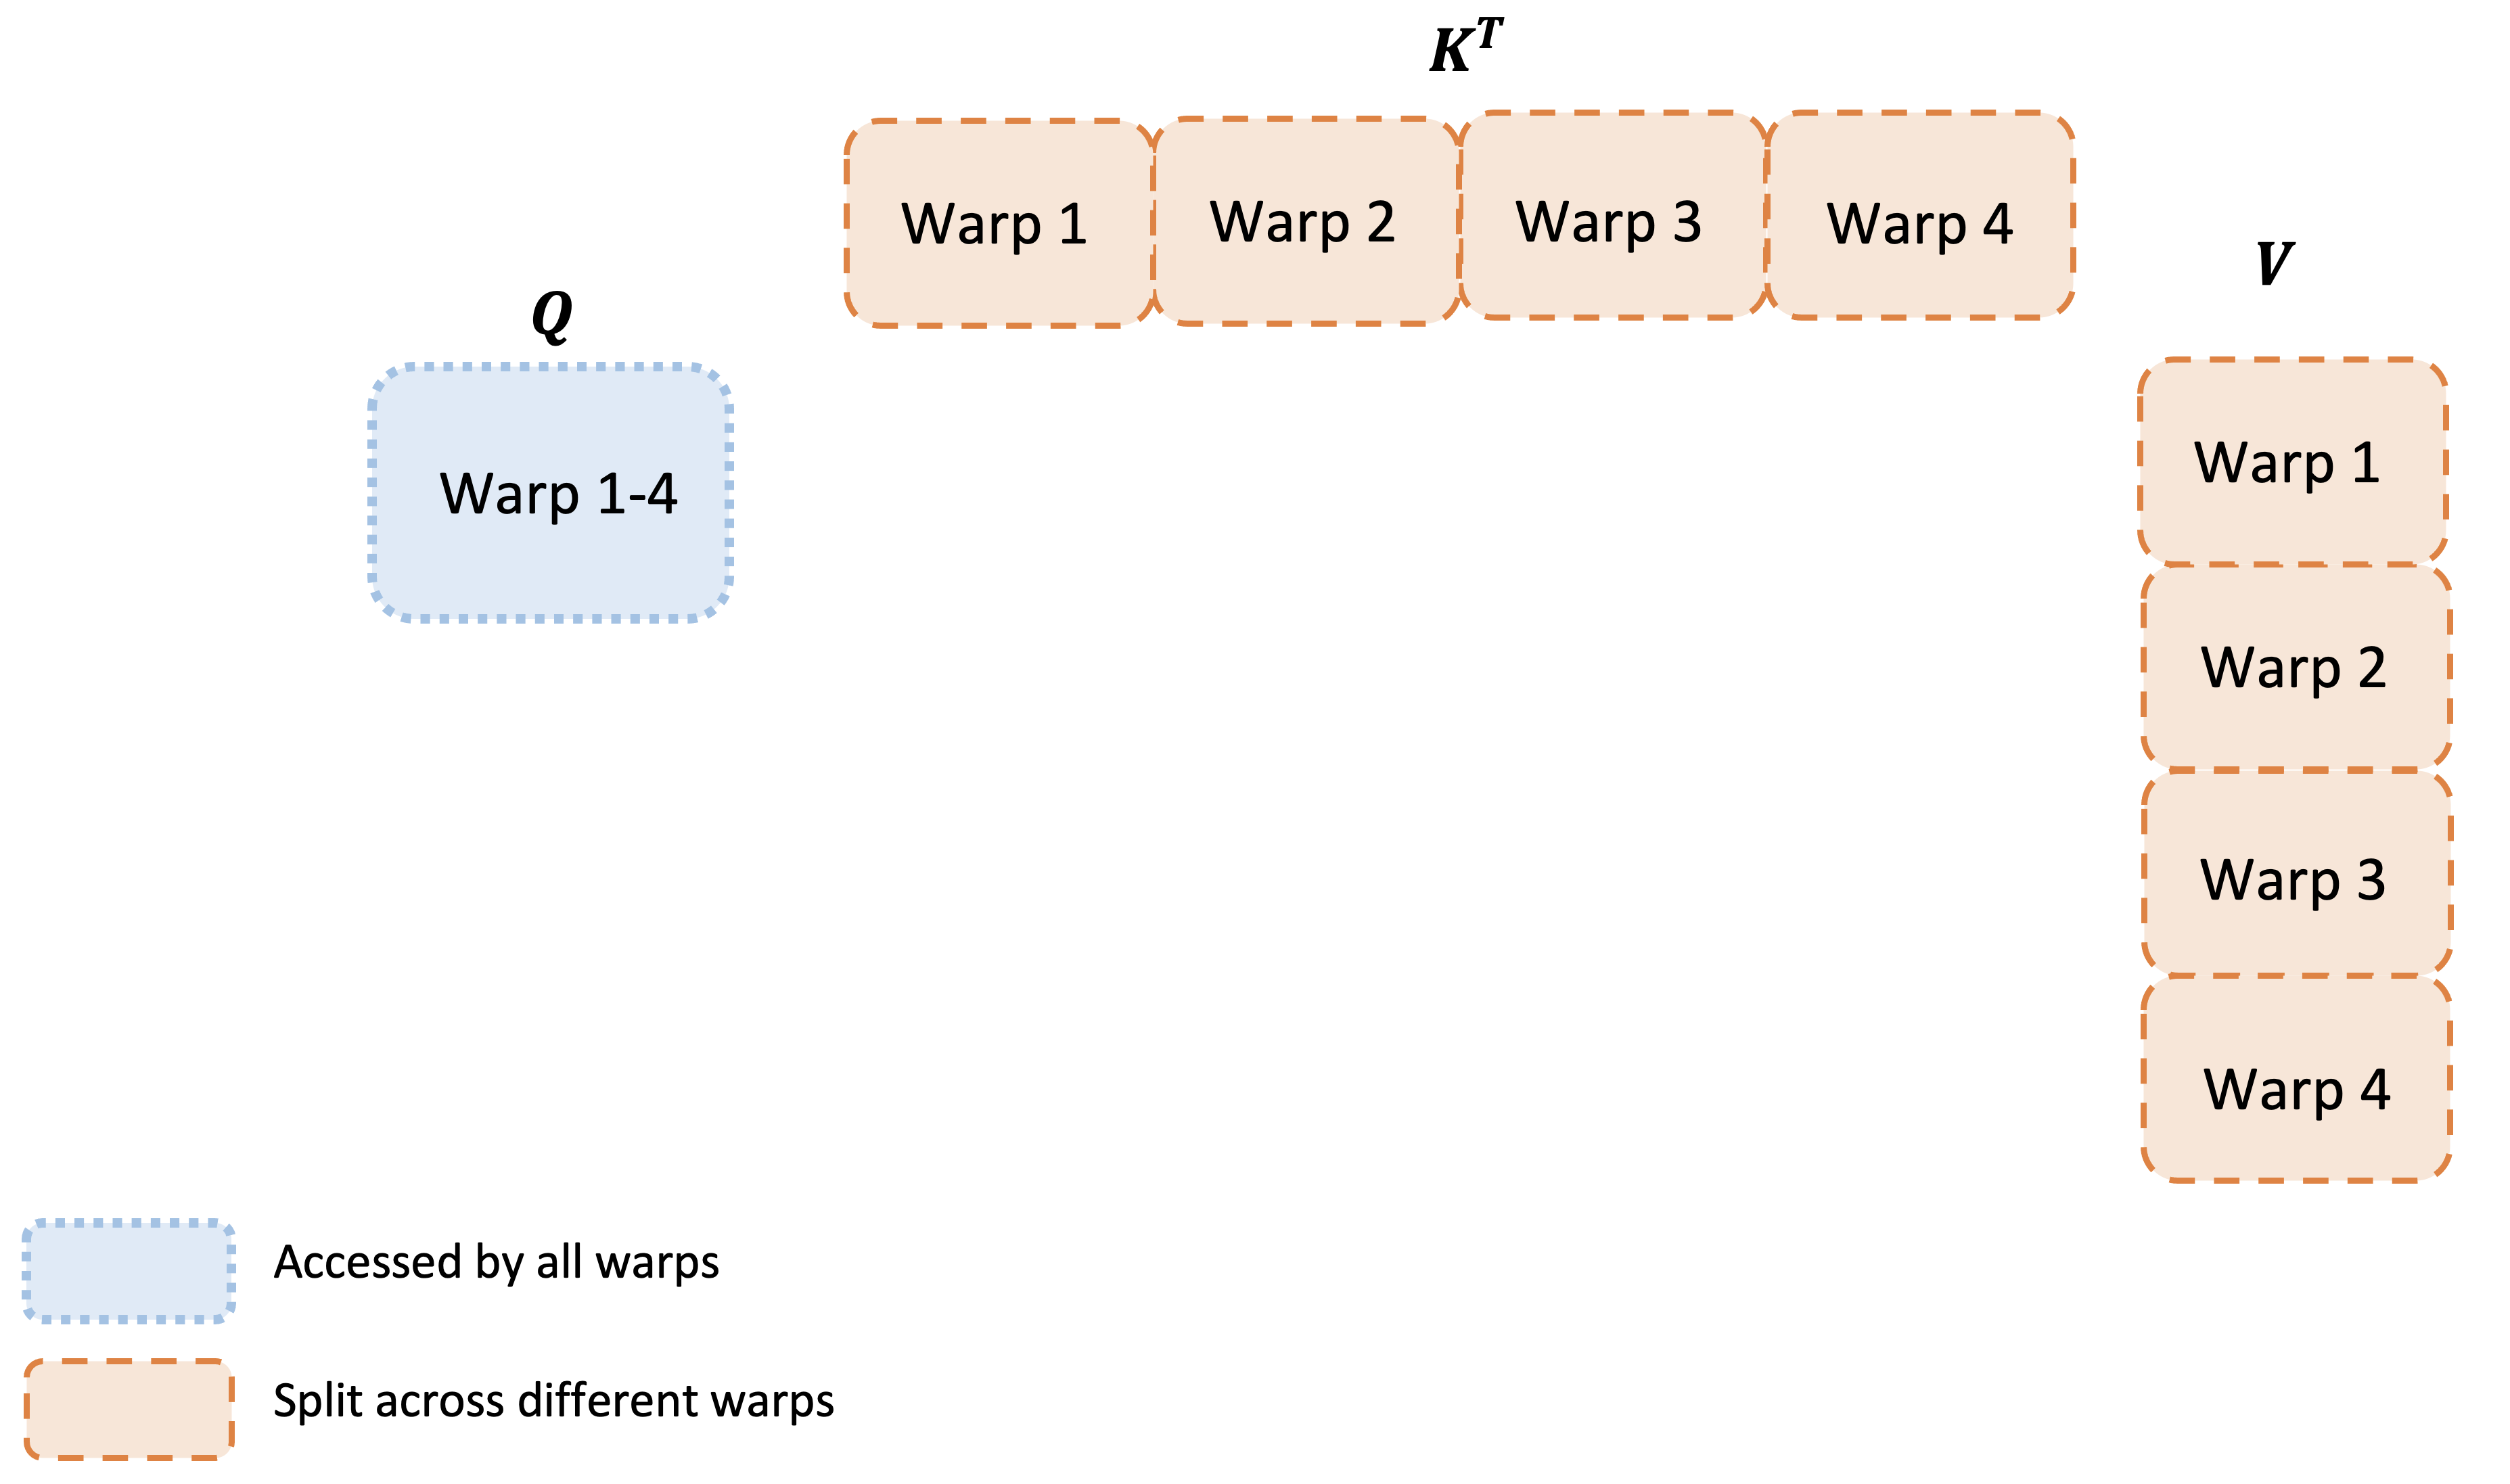
\includegraphics[width=0.47\linewidth]{fa2-fig3a-splitk.png} &
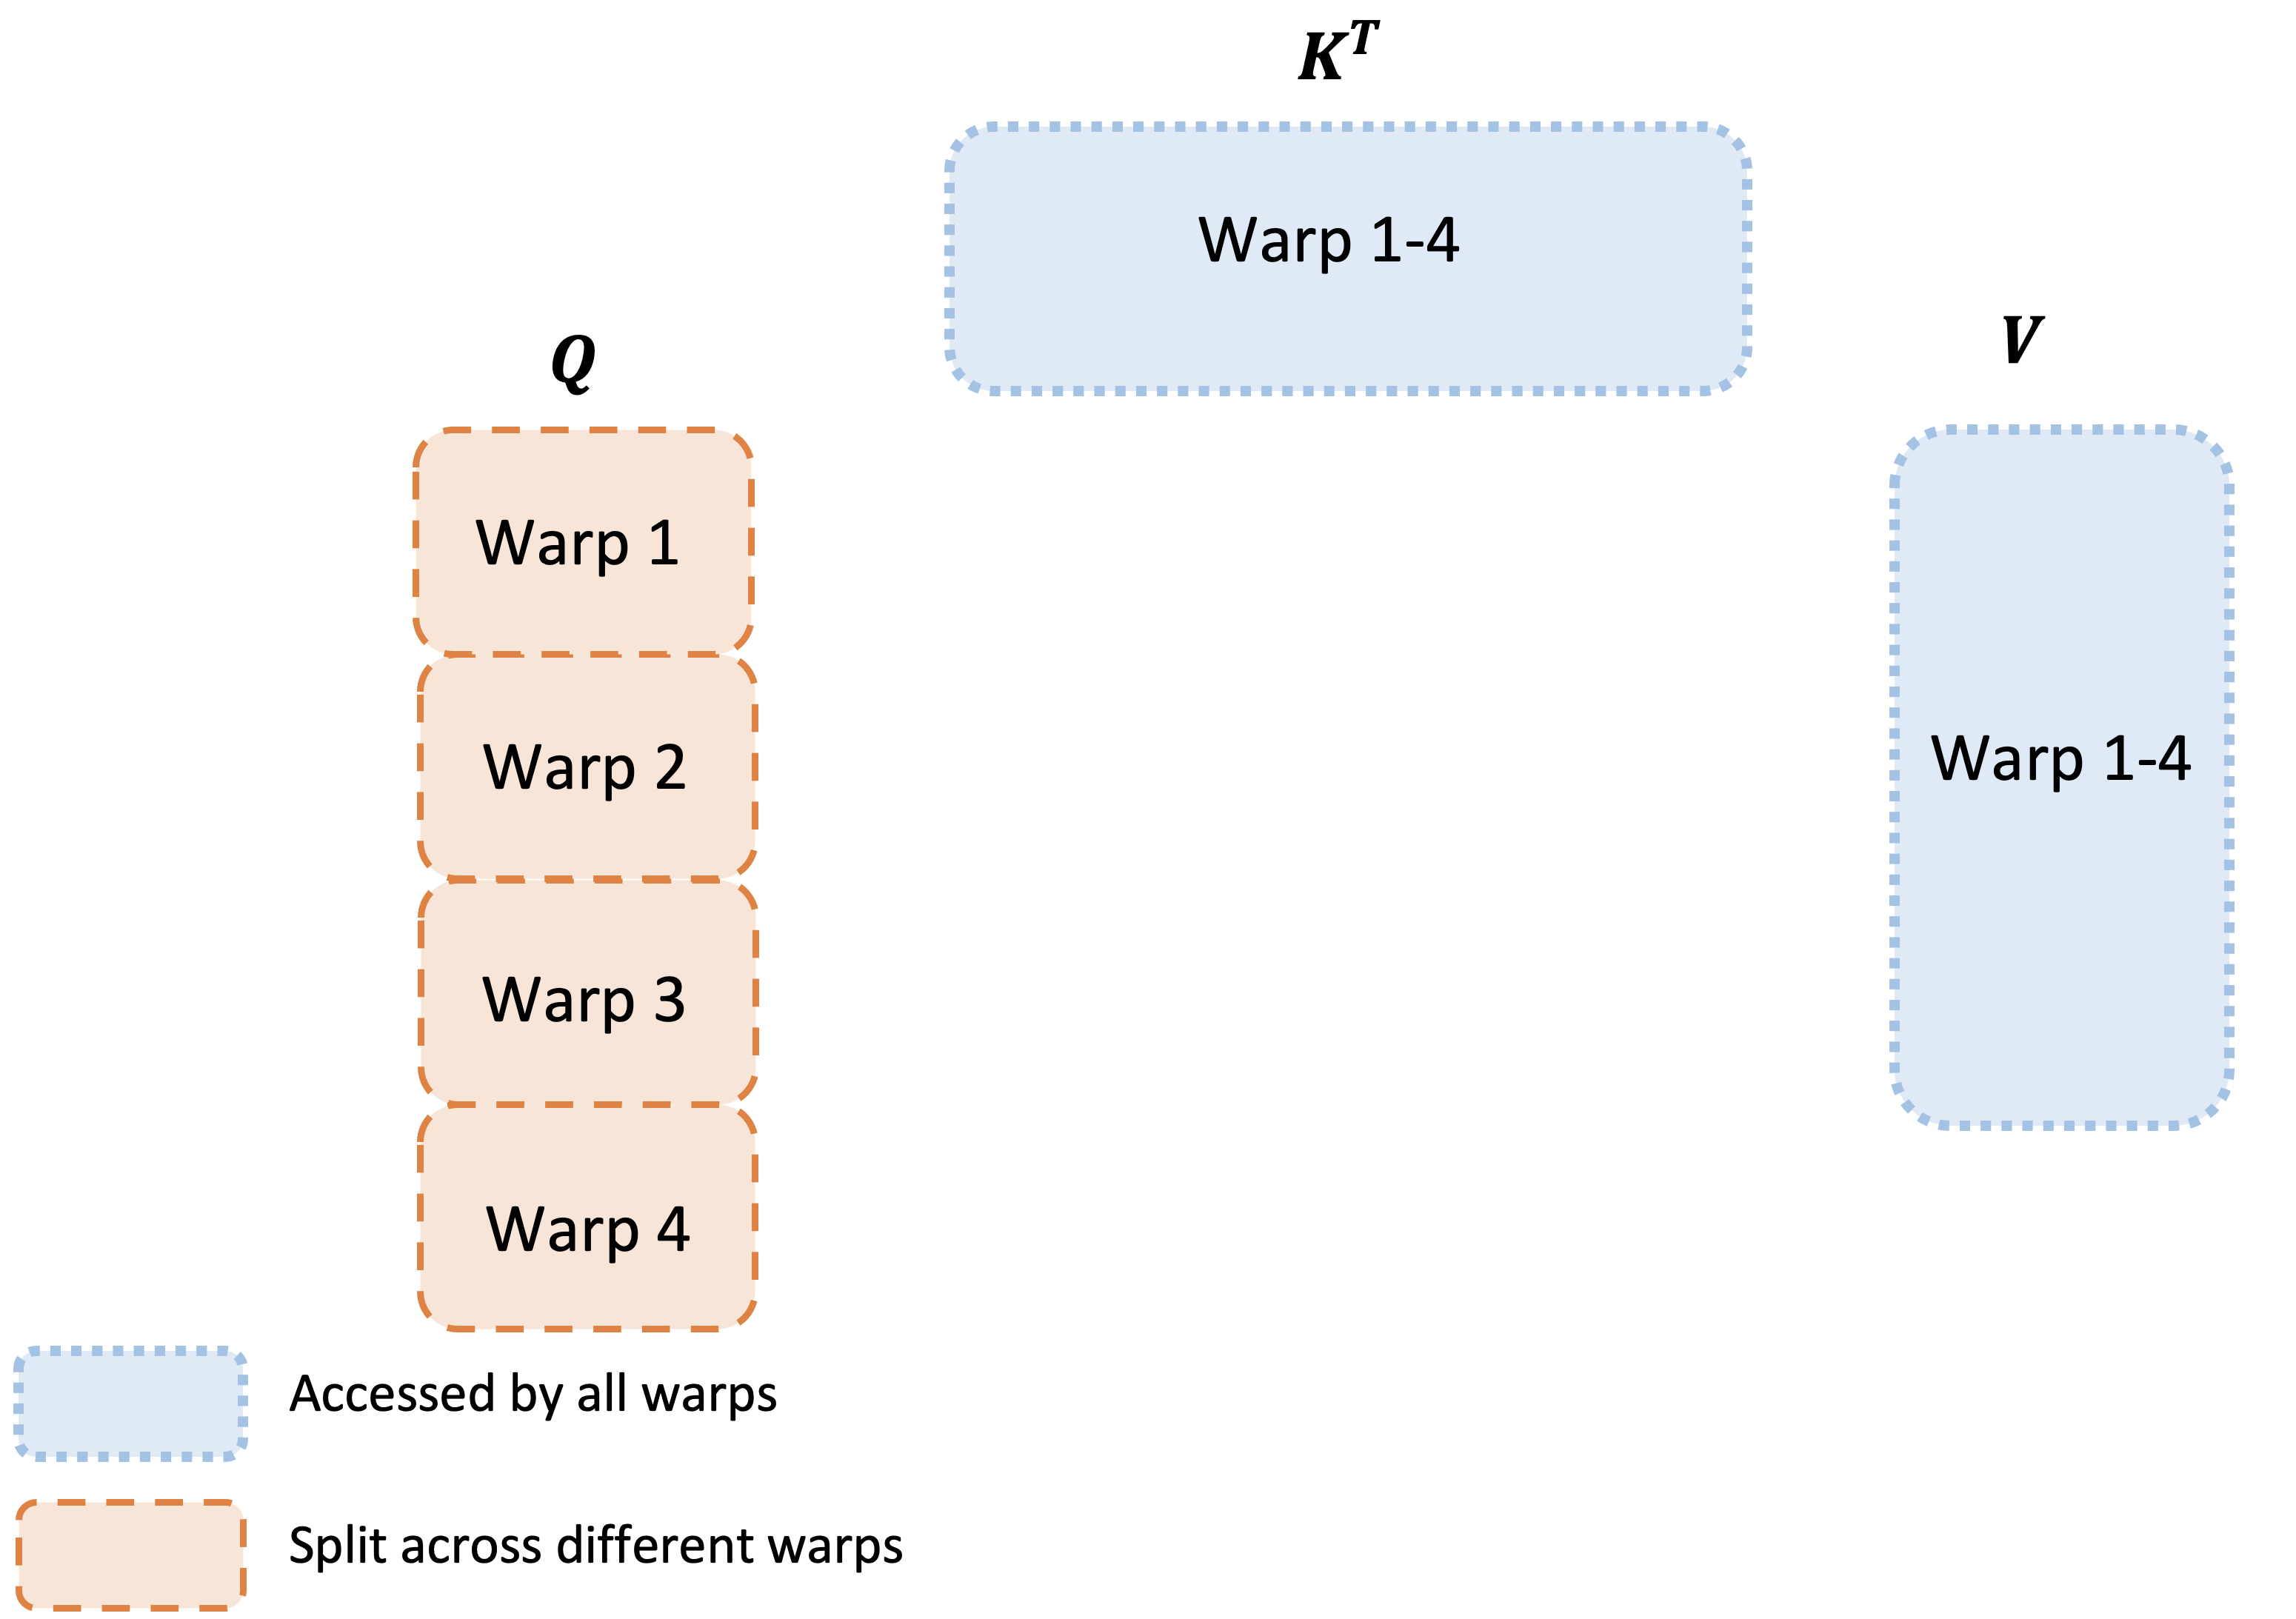
\includegraphics[width=0.47\linewidth]{fa2-fig3b-splitq.png} \\[2pt]
{\small (a) FlashAttention：切 $K/V$} &
{\small (b) FlashAttention-2：切 $Q$}
\end{tabular}
\fignote{论文 Fig.~3：\facite。蓝：所有 warp 共享；橙：切到不同 warp。}
\end{center}

\src{kernel/triton/tutorial/06_attention/step04_flash_causal_mha.py}{67}{80}{加速 FA：Q 块并行与 GQA GROUP}

\figgqa

\texttt{llm\_train} 走加速版。先把教学版的数据流搞懂，再看这些并行与 GQA 改动。

\section{RoPE、GQA、MLA}

RoPE 在 \pyfile{step05_rope.py}，按 head dim 旋转。GQA 是 $H_q>H_{kv}$：推理可用 \pyfile{step06_gqa.py} 的前向 \texttt{flash\_attention\_gqa}；训练必须 \texttt{flash\_attention\_gqa\_train}（有图）。MLA 在 \pyfile{step07_mla.py}，教学版吸收仍偏 Host。

\section{怎么跑}

\begin{runcmd}
\begin{lstlisting}[style=shell]
python kernel/triton/tutorial/06_attention/step01_naive.py
python kernel/triton/tutorial/06_attention/step02_mha.py
python kernel/triton/tutorial/06_attention/step03_flash_single.py
python kernel/triton/tutorial/06_attention/step04_flash_causal_mha_teach.py
python kernel/triton/tutorial/06_attention/step04_flash_causal_mha.py
python kernel/triton/tutorial/06_attention/step05_rope.py
python kernel/triton/tutorial/06_attention/step06_gqa.py
\end{lstlisting}
\end{runcmd}

\section{正确性}

\begin{note}
fwd 教学默认 fp32，$\mathrm{rtol}=10^{-2}$。\texttt{lse} 是 $(B,H,S)$，不要和 4D 的 $O$ 比 shape。反向 smem 比正向紧：同时驻留 $Q,K,V,O,\mathrm{d}O$ 和 tile 上的 $P,\mathrm{d}S$。$64\times 64\times D$ 在本机曾 \texttt{OutOfResources}，教学反向默认 $32\times 32$。
\end{note}

\section{效果}

\begin{remark}
Flash 省的是 HBM 上的 $S/P$，FLOPs 并不更少。墙钟是否赢 SDPA 取决于形状和是否走库函数 Flash。看 launch 次数去做下一章。
\end{remark}

\chapter{用 nsys 看 Launch}

\begin{introduction}
  \item launch $=$ 一次 \texttt{kernel[grid]}
  \item 看名字和次数
  \item 教学 FA 的 $D$ 太大炸 smem
  \item 脚本：\texttt{run\_nsys.sh}
\end{introduction}

配套：\pyfile{kernel/triton/tutorial/07_profiling/}。依赖：先做完第~8~章 Flash。本机 \texttt{torch.profiler} 的 CUPTI 常常采不到 GPU，主线是 \texttt{nsys}。\texttt{ncu} 本课不做。

\section{看什么}

一次 \texttt{kernel[grid](...)} 就是一次 launch。多头不要 Python \texttt{for h} 调 $H$ 次。nsys 首先看 \textbf{kernel 名字和次数}，不要只盯总微秒是否赢 SDPA。

\figlaunch

对照三种实现：PyTorch、naive attention、教学 Flash。形状先用默认 $D=64$。教学 Flash 把整段 $D$ 放进 SRAM，$D=512$ 会因 smem 跑不了，那不是 nsys 坏了。

\section{怎么跑}

\begin{runcmd}
\begin{lstlisting}[style=shell]
source .venv/bin/activate
bash kernel/triton/tutorial/07_profiling/run_nsys.sh
\end{lstlisting}
\end{runcmd}

或手动：

\begin{runcmd}[手动 nsys]
\begin{lstlisting}[style=shell]
cd kernel/triton/tutorial/07_profiling
nsys profile --stats=true --force-overwrite=true \
  --trace=cuda,nvtx,osrt \
  -o nsys_out/flash \
  python nsys_targets.py --impl flash
\end{lstlisting}
\end{runcmd}

\texttt{--impl}：\texttt{torch} / \texttt{naive} / \texttt{flash}。脚本结束会写 \pyfile{nsys_out/compare.md}。

\section{正确性}

\begin{note}
profiling 不替代数值对照。先保证第~8~章 \texttt{allclose}，再采时间。换形状时三种实现用同一 $B,S,D$。
\end{note}

\section{效果}

\begin{remark}
常见结论（以你机器打印为准）：naive 多次 GEMM + softmax，launch 多、中间张量大；Flash 把内层留在一个 kernel。SDPA 可能走完全不同的后端，总时间更短并不矛盾。
\end{remark}

\chapter{推理实战：接到 Qwen3.5}

\begin{introduction}
  \item 0.8B 混合架构
  \item 只换 RMS / SwiGLU / GQA
  \item 裸 kernel，无计算图
  \item 和 vLLM 比的是调度
\end{introduction}

配套：\pyfile{projects/qwen35_infer/}。一条 \textbf{generate}：prefill 整段 prompt，decode 时维护 KV。不要在这里写迷你 vLLM。

\section{公式与数据流}

\texttt{Qwen/Qwen3.5-0.8B} 不是纯 Transformer：24 层大致是 $6\times\bigl(3\times(\text{Gated DeltaNet}\to\mathrm{FFN}) + 1\times(\text{Gated Attention}\to\mathrm{FFN})\bigr)$，大约 18 层线性注意力 + 6 层 softmax 注意力（GQA，$8$ 个 Q 头 / $2$ 个 KV 头，$\mathrm{head\_dim}=256$）。第一版 \textbf{DeltaNet 仍用 PyTorch}（玩具模型里用一层 Linear 占位）。

本课只换三处前向：

\begin{itemize}
  \item RMSNorm：\texttt{rmsnorm}
  \item SwiGLU MLP：\texttt{swiglu\_pro} 再 \texttt{@ W\_down}
  \item GQA Flash：\texttt{flash\_attention\_gqa}，RoPE 用 \texttt{apply\_rope\_offset}
\end{itemize}

\src{projects/qwen35_infer/kernels.py}{14}{20}{推理侧把课上的前向 API 串起来}

\begin{proposition}{没有图}
这些是\textbf{裸 Triton 前向}，没有 autograd 图，不能拿去训练。8GB 不要一上来 bf16 4B/9B；0.8B 短上下文够用。官方 256K 上下文本课不跑。
\end{proposition}

\section{怎么跑}

基础环境见仓库根 README。本目录额外可装 \texttt{transformers}；vLLM 体积大，WSL 上可能难装，不是验收必选项。

\begin{runcmd}
\begin{lstlisting}[style=shell]
python projects/qwen35_infer/smoke_test.py
python projects/qwen35_infer/generate.py --backend toy --kernels eager
python projects/qwen35_infer/generate.py --backend toy --kernels triton
python projects/qwen35_infer/bench.py --backend-list toy_eager,toy_triton
\end{lstlisting}
\end{runcmd}

有权重时再加 HuggingFace / vLLM 对照，短上下文（256--1024）。

\section{正确性}

\begin{note}
同一权重、同一组短 prompt、greedy、相同 \texttt{max\_new\_tokens}。先看文本 / token 是否一致，再看 TTFT、decode tok/s、峰值显存。玩具模型不下载权重也能做核对齐。
\end{note}

\section{效果}

\begin{remark}
vLLM 通常更快，因为 PagedAttention、continuous batching、CUDA Graph 和调度，不是某一个 Softmax 核。课的结论应是：换核后这一层相对 eager 快了多少，端到端还慢在哪。
\end{remark}

\chapter{训练对照：Function 与三后端}

\begin{introduction}
  \item 必须 \texttt{Function.apply}
  \item 默认只换 FA
  \item Adam 不被 autocast 减掉
  \item \texttt{compile} 常赢端到端
\end{introduction}

配套：\pyfile{projects/llm_train/}。架构是 \textbf{LayerNorm + RoPE + GQA + SwiGLU}（训练骨架用 LN，不是 RMSNorm），不是 Qwen3.5 的 DeltaNet。只跑若干 step：看 step 时间、tok/s、峰值显存、loss 是否同量级，不训到可用 chatbot。

\section{公式与数据流}

推理可以调裸前向；训练必须 \texttt{torch.autograd.Function}。\texttt{Function.apply} 才建图，自己调 \texttt{forward} 不会进 \texttt{backward}。\texttt{save\_for\_backward} 只存反向真正用到的量：Softmax 存 $y$ 不存 $x$；Flash 存 $Q,K,V,O,\mathrm{LSE}$，不能存完整 $P$。

默认 \texttt{--triton-ops fa}：只换 FlashAttention，LN 与 MLP 仍走 PyTorch / cuBLAS。

\figtrainops

\begin{lstlisting}[style=shell]
hidden -> F.layer_norm -> FA Function (GROUP) -> residual
       -> F.layer_norm -> silu(x@Wg)*(x@Wu) + Linear down -> residual
\end{lstlisting}

教学对照再开 \texttt{--triton-ops fa,ln,swiglu}。MLP 的 down 始终 \texttt{nn.Linear}。教学大 GEMM 打不过 cuBLAS，开了会负优化。

\src{projects/llm_train/kernels.py}{31}{54}{训练默认只换 FA；LN / SwiGLU 需显式打开}

\subsection{显存账}

\begin{proposition}{Adam 不在 autocast 里}
混合精度（\texttt{autocast} bf16）\textbf{减的是激活和 matmul，不是 Adam 状态}。约 1B 参数全参 AdamW：权重 bf16 约 2~GB，Adam $m/v$ 常仍是 fp32 约 8~GB，再加梯度与激活。\textbf{8GB 笔记本全参 1B 会 OOM}。默认 \texttt{--config small}（约 0.25B，$\mathrm{seq}=256$）；\texttt{1b} 失败时看脚本打印的账即可，不算课程失败。
\end{proposition}

\section{怎么跑}

\begin{runcmd}
\begin{lstlisting}[style=shell]
python projects/llm_train/train.py --config small --backend eager --steps 5
python projects/llm_train/speed.py --config small --steps 20
python projects/llm_train/bench.py --config small --steps 10
\end{lstlisting}
\end{runcmd}

Triton tile 在 \pyfile{projects/llm_train/tiles.py}，或命令行 \texttt{--fa-block-m} 等覆盖。显式 launch 必须带 \texttt{num\_stages}，否则 JIT 默认 3 级流水会把 smem 乘过本机上限。FA 反向不要上 $64\times 64$。

\section{正确性}

\begin{note}
loss 同量级即可，不要求 bit 级一致。裸 kernel 没有 \texttt{grad\_fn}；autocast 下 $QKV$ 常是 bf16、交叉熵回传的 $\mathrm{d}O$ 常是 fp32，\texttt{tl.dot} 要求两侧同 dtype，加速 FA 会把 $\mathrm{d}O$ cast 到 $Q$ 的 dtype。
\end{note}

\section{效果}

三后端：

\begin{table}[htbp]
  \centering
  \caption{训练对照里实际在跑什么}
  \begin{tabular}{ll}
    \toprule
    后端 & 实现 \\
    \midrule
    \texttt{eager} & \texttt{F.layer\_norm} + SDPA(\texttt{enable\_gqa}) + silu GEMM \\
    \texttt{compile} & 同一套 eager + \texttt{torch.compile} \\
    \texttt{triton}（默认 \texttt{fa}） & 只换 FA；LN / MLP 仍 cuBLAS \\
    \texttt{fa,ln,swiglu} & 再换教学 LN / 融合 SwiGLU \\
    \bottomrule
  \end{tabular}
\end{table}

\begin{conclusion}
\texttt{compile} 常赢端到端。Triton 默认只比 FA 对 SDPA；不要用教学 Linear 去和 cuBLAS 比整步时间。数字以你机器 \texttt{speed.py} 为准。
\end{conclusion}


\appendix
\chapter{容易踩的坑}

下面从课上反复出现的问题里抽出仍有效的条目，不按作者进度板逐条抄。

\begin{problemset}[课上反复出现的坑]
  \item \textbf{归约维}（最后一维）不能随意用 \texttt{program\_id} 切开；要么整行装下，要么 program 内 \texttt{for} 合并统计量。
  \item Online Softmax / 分块 Norm 往往是为了 $N$ 很大或为 Flash 铺路；单独写出完整 Softmax 时 online 不一定更快。
  \item Naive 整行 \texttt{BLOCK\_N = next\_power\_of\_2(N)} 在 $N=8192$ 时会寄存器爆炸。
  \item 对照要公平：TF32、\texttt{synchronize}、warmup。
  \item \texttt{@triton.jit} 里不能调 Python wrapper；组合算子在 Host 串调用。Host 串多次 launch \textbf{不算} kernel 融合。
  \item 3D matmul 接多头：$(B,H,S,d)$ 先展成 $(BH,S,d)$。Flash 多头则 \texttt{grid=(B,H)}，基址加 \texttt{stride\_h}。
  \item \texttt{atomic\_add} + autotune 必须 \texttt{reset\_to\_zero}。
  \item SDPA $\ne$ 单一 Flash：对照用 \texttt{scaled\_dot\_product\_attention}。
  \item FA2 是双循环：外 $Q$、内 $K/V$。内层必须 \texttt{for}。
  \item Launch $=$ 一次 \texttt{kernel[grid](...)}。不要 Python \texttt{for h}。
  \item Causal 加在 \texttt{qk} 上（\texttt{offs\_n <= offs\_m}），不是 load 的越界 mask。Triton 没有 \texttt{break}。
  \item Head dim 用 64/128。教学核 $D$ 太大炸 smem（本机上限约 $101376$）。
  \item 有 \texttt{@triton.autotune} 就不要再传 \texttt{BLOCK\_*}；\texttt{grid} 用 \texttt{lambda meta}。转置是 \texttt{tl.trans} 不是 \texttt{tl.transpose}。
  \item Triton kernel 不进计算图，必须 \texttt{Function}。\texttt{apply} 才建图。
  \item \texttt{save\_for\_backward} 只存反向要用的量。Flash 不能存完整 $P$。
  \item 裸输出没有 \texttt{grad\_fn}。对照用 \texttt{Function.apply} vs SDPA，一次求出 $\mathrm{d}Q,\mathrm{d}K,\mathrm{d}V$。
  \item \texttt{lse} 是 $(B,H,S)$。\texttt{dQ} atomic 必须从零开始。
  \item FA 反向 smem 更紧；教学反向 $32\times 32$。显式 launch 记得 \texttt{num\_stages}。
  \item 跑示例用 \texttt{python path.py}，不要 bash 直接执行没有 shebang 的 \texttt{.py}。
  \item 教学 GEMM / LN 打不过 cuBLAS：训练默认只换 FA。
\end{problemset}

\chapter{符号与文件}

\begin{table}[htbp]
  \centering
  \caption{符号}
  \begin{tabular}{ll}
    \toprule
    符号 & 含义 \\
    \midrule
    $B,H,S,D$ & batch、头数、序列、head dim \\
    $H_q,H_{kv}$ & GQA 的 Q 头与 KV 头 \\
    $m,\ell$ / LSE & 在线 softmax 的行最大值与归一化；$\mathrm{LSE}=m+\log\ell$ \\
    BLOCK\_M/N/K & 输出行块 / 列块 / 归约块 \\
    program / pid & 一次并行实例，接近 CUDA block \\
    SM / warp & GPU 上的计算核心；32 线程锁步调度 \\
    HBM / SRAM & 全局内存 vs SM 上的 shared memory \\
    \bottomrule
  \end{tabular}
\end{table}

\begin{table}[htbp]
  \centering
  \caption{仓库入口}
  \begin{tabular}{ll}
    \toprule
    路径 & 内容 \\
    \midrule
    \texttt{kernel/triton/tutorial/} & 01--07 算子 \\
    \texttt{.../step04\_flash\_causal\_mha\_teach.py} & 教学 FA \\
    \texttt{.../step04\_flash\_causal\_mha.py} & 加速 FA（训练） \\
    \texttt{projects/qwen35\_infer/} & 推理 generate \\
    \texttt{projects/llm\_train/} & 训练对照 \\
    \texttt{docs/textbook/} & 本书 \\
    \url{https://arxiv.org/abs/2307.08691} & FA2 论文（第~8~章插图出处，勿把 PDF 放进仓库） \\
    \bottomrule
  \end{tabular}
\end{table}

\section*{参考文献}

\noindent\facite。\url{\faurl}。
第~8~章 Fig.~1--3 与 Algorithm~1 直接引自该文，用于对照仓库里的教学 / 加速核。


\end{document}
